%\chapter{Sběr a zpracování velkých dat}\label{kap:bigData}
\chapter{Zpracování velkých dat}\label{kap:bigData}
Získaná data je potřeba zpracovat a vytěžit z~nich co největší množství důležitých informací. Při menším objemu dat se nejedná o~větší problém, ale pokud se bavíme o~velkých datech, u~kterých je potřeba zpracovávat i několik milionů hodnot za vteřinu, nastávají potíže. Programy pro zpracovávání velkých dat jsou obvykle součástí celých systémů pro práci s~velkými daty včetně úložišť, vizualizačních programů a často jsou právě s~úložišti pevně spjaté. Takovým příkladem je Kapacitor, který je součástí platformy Tick, jejíž schéma je vidět na obrázku \ref{pic:tick}. Způsob zpracování také závisí na povaze dat. Nejzákladnějším rozdělením zpracování velkých dat je proudově a blokově orientované.

\section{Proudově orientované zpracování}
Informace o~proudově orientovaném zpracování dat pochází z~\cite{BigDataPlatforms}. Jedná se o~zpracování toku dat v~reálném čase, data jsou tudíž zpracovávána okamžitě při příchodu a ukládají se až po zpracování. V~některých aplikacích data po zpracování ukládána ani nejsou, a to z~důvodu jejich obrovské velikosti. Tento přístup se využívá v~případech, kdy je vyžadována nízká odezva mezi příchodem dat a jejich efektem. Efektem může být výstup v~podobě upozornění pro uživatele. Tato podmínka je kritická pro všechny typy monitorování. Ať už jde o~kontrolu síťového provozu, protipožární ochranu či detekci poruch na průmyslových strojích. Nízká odezva je extrémně důležitá pro rychlé reakce v~případech nenadálých událostí. Tuto podmínku nemůže splnit zpracování po blocích. 

Proudově orientované zpracování musí zajišťovat vysokou dostupnost, aby veškeré události byly ihned zpracovány. Toho se dosahuje pomocí:
\begin{itemize}
    \item distribuce zpracování na několik uzlů a možnosti další škálovatelnosti,
    \item replikace zpracování, při poruše jednoho uzlu lze zachytit událost na jiném uzlu a nedochází ke ztrátě dat,
    \item zpracování ve vnitřní paměti pro dosažení co nejmenší odezvy po příchodu dat a jejich zpracováním, 
    \item paralelního zpracování proudu.
\end{itemize}

Jedním z~příkladů frameworku implementujícího zpracování v~reálném čase je Kapacitor či Apache Spark. Apache Spark poskytuje rozhraní pro psaní programů a jejich distribuci na výpočetních uzlech. Spark zajišťuje toleranci chyb a škálovatelnost stejně jako model MapReduce a může zapisovat do všech databází využívající tento model. Knihovna Spark Streaming poskytuje rozšíření o~možnost zpracovávání dat v~reálném čase s~vysokou propustností. Spark mimo jiné také poskytuje možnost integrace s~nástroji z~Apache hadoop, které jsou původně zaměřené na blokové zpracování dat. 

\section{Blokově orientované zpracování}
Tato metoda zpracovává data po blocích, které již byly shromážděny v~paměti. Nevýhodou tedy je zpoždění získání výsledků analýz z~přijatých dat. Využívá se v~oblastech, kde není potřeba rychlé zpracování hodnot. Například při periodických výpočtech maxim, minim či středních hodnot z~dat uložených v~časových databázích. Jedním z~programů, který poskytuje zpracování po blocích dat čtených z~časové databáze InfluxDB, je Kapacitor. Kapacitor tedy nabízí obě možnosti zpracování dat, je proto vhodný jak pro sledování událostí v~reálném čase, tak pro generování zpráv za delší časové období \cite{batchProcessing}.

\subsection*{MapReduce}
Zdrojem této podsekce je \cite{MapReduce}. Mimo později vyvinutý Apache Spark zmíněný výše je Apache Hadoop primárně zaměřený na zpracovávání dat po blocích. K~tomu využívá framework MapReduce. Jedná se o~programovací model pro zpracování velkého množství dat po blocích pomocí paralelizace a je implementován v~mnoha programovacích jazycích. Celý proces probíhá ve 4 fázích -- rozdělení, mapování, míchání a redukování. Celý postup zpracování jednoho požadavku na výpočet počtu jednotlivých slov ve větě je vidět na obrázku \ref{pic:MapReduce}. Vstupem jednotlivých fází je dvojice klíč-hodnota. Vstup se zpracovává uživatelem definovanou mapovací a redukční funkcí. Jednotlivé fáze provádí:
\begin{itemize}
    \item v~rozdělovací fázi dochází k~rozdělení vstupních dat na formát, který zpracovává mapovací funkce,
    \item mapovací fáze vytvoří výsledek pomocí mapovací funkce, v~našem případě se jedná o~dvojici obsahující slovo a počet výskytů toho slova,
    \item následně při míchání dochází k~setřídění výsledků,
    \item a v~poslední fázi redukce dojde k~agregaci a odeslání výsledku uživateli.
\end{itemize}

\begin{figure}[h]
  \centering
  \scalebox{0.39}{
        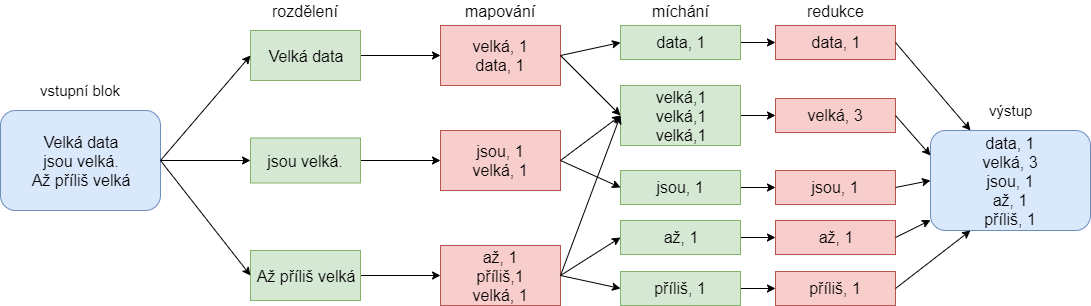
\includegraphics{obrazky-figures/mapReduce.png}
    }
  \caption{Příklad MapReduce modelu pro počítání výskytu jednotlivých slov \cite{MapReduce}.}\label{pic:MapReduce}
\end{figure}

V~praxi je framework MapReduce distribuovaný, tudíž obsahuje více uzlů. Jeden ze serverů přijme požadavek a rozešle úkoly na provedení Map a Reduce funkcí na ostatní uzly. Kvůli zamezení výpadku může provádět i duplicitní výpočet na více uzlech. Po získání výsledků provede dotázaný server zahození duplicitních mezivýsledků a odešle odpověď klientovi.

\section{Zpracování dat ze senzorů vibrací}\label{sec:vibrationAggregation}
%Root mean square, delta treshold, FIR a IIR filtr
Tato sekce čerpá z~\cite{vibrationData}. Pro data z~vibrací je důležitá funkce kvadratického průměru. Kvadratický průměr neboli RMS (Root Mean Square) se vztahuje k~energii vibrací a je důležitým faktorem pro monitorování stavu strojů. Vzorec kvadratického průměru pro blok hodnot je: 
\begin{eqnarray}\label{eq:root_mean_square}
  x_{rms} & = & \sqrt{\frac{\sum_{i=1}^{n} x_i^2}{n}}
\end{eqnarray}
kde $n$ je počet vzorků v~bloku, a $x_n$ je hodnota n-tého vzorku. Dále je pro data z~vibrací důležitá maximální amplituda signálu a Rychlá Furierova Transformace. Rychlá Furierova Transformace se používá pro frekvenční analýzu vibrací která dokáže odhalit abnormální vibrace stroje způsobené poškozením určité součástky.

\section{Komprese dat}\label{sec:compression}
Velká data mohou nabývat velikosti petabajtů nebo i více a je neefektivní je udržovat v~nekomprimované podobě. Ať už jde o~omezení síťové komunikace, či udržování dat na úložišti, je vhodné do určité míry omezit jejich velikost. Zároveň je nutné myslet na budoucí využití komprimovaných dat. Pokud mají být data rychle k~dispozici pro provádění analýz nebo vizualizaci, musí být dekomprimace dat rychlá. Tato sekce se zaměřuje na popis metod využitelných pro body obsahující kombinaci celočíselné časové značky a naměřené desetinné hodnoty. Komprese tohoto formátu je potřebná při čtení a zpracování dat ze senzorů při monitorování strojů, na což je tato práce zaměřená.

\subsection{Delta encoding}\label{sec:delta}
Komprese pomocí metody delta encoding je vhodná pro pravidelně či málo se měnící hodnoty celých čísel, jako je unixová časová značka. Metoda je založená na výpočtu rozdílu sousedních hodnot, vzorec pro výpočet je následující \cite{smith2003digital}:
\begin{eqnarray}\label{eq:delta}
  \Delta_t & = & t_n-t_{n-1}
\end{eqnarray}
Touto metodou může dojít ke snížení rozsahu hodnoty nutné k~uložení čísla. V~případě unixové 32bitové časové značky, která je zaznamenávána při pravidelném měření, může dojít k~citelné kompresi dat. Příklad je možné vidět v~tabulce \ref{tab:delta}. První sloupec tabulky obsahuje nekomprimované časové značky o~velikosti 32 bitů. V~druhém sloupci se nachází $\Delta t$ těchto hodnot. První bod se pouze přesune z~důvodu zachování počátečního bodu a nedojde tedy k~jeho kompresi. K~uložení rozdílů, které v~tomto případě nabývají pouze kladných hodnot, postačí 6 bitů poskytujících rozsah $0\textup{--}127$. Čím výraznější změna mezi hodnotami nastává, tím horších výsledků je dosaženo. Tato metoda tedy nemá smysl pro kompresi například řetězce ASCII znaků. Jak lze vidět na sloupci $\Delta ASCII$, výsledky nabývají i záporných hodnot. K~zakódování jednoho znaku bychom potřebovali 8 bitů. Jelikož je ASCII znak reprezentován 8bitovou hodnotou, nebylo by dosaženo žádného zlepšení \cite{smith2003digital}.

Časová databáze Gorilla (viz \ref{sec:gorilla}) využívá pro kompresi časových značek pozměněnou verzi této metody založenou na podmínce, že měření se opakuje v~pravidelných intervalech. Vzorec \ref{eq:deltadelta} tedy odečítá deltu předchozích hodnot od delty aktuálních hodnot. Hodnoty jsou ukládané po dvouhodinových blocích. Hlavička obsahuje časovou značku zarovnanou na začátek daného dvouhodinového bloku a první delta využívá původní vzorec \ref{eq:delta}, kde $t_{n-1}$ je časová značka z~hlavičky. Hodnoty jsou následně ukládány s~proměnlivou délkou\cite{gorilla}. 
\begin{eqnarray}\label{eq:deltadelta}
  D & = & (t_n-t_{n-1})-(t_{n-1}-t_{n-2})
\end{eqnarray}
Možnost využití této úpravy je viditelná i na vzorových datech v~tabulce \ref{tab:delta}, kde měření probíhá zhruba jednou za minutu. Jak je vidět ve sloupci $\Delta\Delta t$ (počáteční hodnota zarovnaná na začátek dvouhodinového intervalu činí 1577664000), oproti předchozí verzi metody došlo ke kompresi první hodnoty z~32 na 5 bitů a zbylé hodnoty je možné uložit na 4 bitech.

\begin{table}[h]
    \begin{center}
        \begin{tabular}{|c|c|c||c|c|c|}
        \hline
             časová značka & $\Delta t$ & $\Delta\Delta t$ & znak & ASCII hodnota & $\Delta ASCII$ \\ \hline
             1577664060 & 1577664060 & 60 & B & 66 & 66 \\
             1577664120 & 60 & 0 & i & 105 & 39 \\
             1577664178 & 58 & -2 & g & 103 & -2 \\
             1577664239 & 61 & 3 & D & 68 & -35 \\
             1577664302 & 63 & 2 & a & 97 & 29 \\
             1577664361 & 59 & -4 & t & 116 & 19 \\
             1577664425 & 64 & 5 & a & 97 & -19 \\ \hline
        \end{tabular}
        \caption{Příklad výpočtu komprimovaných hodnot Delta encoding pro pravidelné časové značky a řetězec znaků.} \label{tab:delta}
    \end{center}
\end{table}
\subsection{XOR encoding}\label{sec:xor}
Teoretické informace této podsekce pochází z~\cite{gorilla}. Metodu využívá časová databáze Gorilla (viz \ref{sec:gorilla}) pro kompresi desetinných čísel s~dvojitou přesností. XOR encoding funguje na podobném principu delta komprese - ukládá rozdíl sousedních hodnot. Základem metody je operace $\oplus$ (XOR) mezi dvěma po sobě jdoucími čísly. Hodnoty jsou ukládány podle následujících pravidel:

\begin{enumerate}
    \item první hodnota je uložena bez komprese,
    \item pokud je výsledek operace $\oplus$ 0 (hodnoty jsou totožné), uloží se pouze jeden nulový bit,
    \item pokud je výsledek operace $\oplus$ nenulový (hodnoty se liší) a zároveň počet nulových bitů na začátku a konci výsledku \textbf{je} stejný nebo vyšší než u~předchozího výsledku, jako první se uloží kontrolní bity $10$ následované nenulovou částí výsledku operace,
    \item pokud je výsledek operace $\oplus$ nenulový (hodnoty se liší) a zároveň počet nulových bitů na začátku a konci výsledku \textbf{není} stejný nebo vyšší než u~předchozího výsledku, jako první se uloží kontrolní bity $11$, následuje 5 bitů obsahující počet počátečních nul, 6 bitů obsahující délku nenulových bitů a samotné nenulové bity výsledku.
\end{enumerate}

Příklad reprezentace všech tří možností uložení v~paměti je možné vidět v~tabulce \ref{tab:xor}. První hodnota v~paměti je opsána podle pravidla číslo jedna. U~druhé hodnoty nedošlo ke změně, a proto je uložen pouze jeden bit prefixu (prefixy jsou označeny červeně) obsahující nulu podle druhého pravidla. U~třetí hodnoty došlo ke změně, a jelikož je počet nul před a po nenulových bitech nižší (předchozí hodnota má všechny bity nulové), je použito čtvrté pravidlo. První dva bity určují prefix, následujících 5 bitů vyznačených modře označuje počet nulových bitů před hodnotou, 6 bitů označených zeleně obsahuje délku výsledku a poslední je samotný výsledek operace. Čtvrté číslo je uloženo v~paměti pomocí třetího pravidla, protože počet nul před výsledkem je totožný jako u~předchozího a počet nul za výsledkem je o~jednu vyšší. První dva bity opět označují prefix a zbytek obsahuje výsledek.

\begin{table}[h]
 \footnotesize
 \begin{center}
    \begin{tabular}{|c|c|c|c|c|}
        \hline
         dec & hex & $\oplus$ s~předchozí & uloženo v~paměti & velikost [b] \\ \hline
         $19.0625$ & 0x4033100000000000 & - & 0x4033100000000000 & 64 \\
         $19.0625$ & 0x4033100000000000 & 0x0 & $0b$\textcolor{red}{0} & 1 \\
         $41.25$ & 0x4044A00000000000 & 0x0077B00000000000 & 0b\textcolor{red}{11}\textcolor{blue}{01001}\textcolor{green}{001010}11101111011 & 24 \\
         $25.5$ & 0x4039800000000000 & 0x007D200000000000 & 0b\textcolor{red}{10}11111010010 & $13$ \\ \hline
        \end{tabular}
    \caption{Příklad výpočtu komprimovaných hodnot pro XOR encoding.} \label{tab:xor}
    \end{center}
\end{table}

Hlavní výhodou metody je nutnost pouze jednoho bitu k~uložení nezměněné hodnoty a při menších změnách dosahuje několikanásobné komprese. Metoda je tedy vhodná například pro data pořízená z~měření teploty, u~kterých nedochází k~velkým výkyvům. 

\section{Síťová komunikace a zabezpečení} \label{sec:networkComm}
 Mnoho zařízení pro monitorování vzniklých před nebo v~počátcích čtvrté průmyslové revoluce disponuje proprietárními komunikačními protokoly. Tyto protokoly jsou neveřejné a výrazně omezují větší změny v~systému, jako je nákup zařízení od jiných výrobců či napojení na novější systémy. Postupem času začaly vznikat otevřené standardy jako je MODBUS TCP či EtherCAT pro lokální komunikaci. Upuštění od proprietárních komunikačních protokolů tedy značně usnadňuje vytvoření a propojení systémů IIoT (Industrial internet of things) od různých výrobců do jednoho celku.

MODBUS je bitově orientovaný asynchronní komunikační protokol využívající TCP, určený pro výměnu informací mezi vestavěnými systémy a průmyslovými aplikacemi. Protokol využívá takzvaný \textit{pooling} neboli aktivní dotazování metodou dotaz-odpověď. Pomocí dotazu si lze vyžádat data či provést příkaz. Odpověď obsahuje potvrzení provedení vyžadovaného příkazu či vyžádaná data. Další protokol, který se využívá, je MQTT. Jedná se opět o~TCP protokol, je oproti protokolu MODBUS synchronní a využívá model \textit{publisher–subscriber} (vydavatel-odběratel). O~výměnu zpráv se stará jeden centrální bod zvaný MQTT broker. Ten zprávy přijímá od vydavatelů, třídí do takzvaných témat a rozesílá všem odběratelům, kteří jsou k~danému tématu přihlášeni \cite{iotComm}. 

Standardizované protokoly nejsou vhodné pro každé využití. Jsou určeny spíše pro informování o~změně stavu v~lokální síti a ne pro zasílání velkého množství dat pro zpracování přes internet. Protokoly vyžadují výměnu mnoha zpráv, takzvaných \textit{handshake} zpráv, před zasláním samotné zprávy s~informacemi, a nejsou zabezpečeny. Pro zasílání většího množství zpráv přes internet je vhodnější využít vlastních zjednodušených a zabezpečených UDP či TCP protokolů. Komunikaci přes TCP lze zabezpečit pomocí SSL (Secure Sockets Layer) certifikátu, který vytváří šifrované spojení.
%https://sites.google.com/site/amitsciscozone/home/security/ssl-connection-setup
UDP pakety lze zabezpečit například pomocí DTLS (Datagram Transport Layer
Security) či jednoduchou bitovou operací XOR.
%https://tools.ietf.org/html/rfc6347


%https://www.researchgate.net/publication/331588782_Communication_Protocols_of_an_Industrial_Internet_of_Things_Environment_A_Comparative_Study

\section{Vizualizace a vyhodnocení velkých dat ze senzorů}
Vizualizace dat ze senzorů při využití existujících řešení často úzce souvisí se zvoleným úložištěm. Téměř každé úložiště velkých dat je možné propojit s~nějakou vizualizační aplikací. Jednou z~nejrozšířenějších vizualizačních aplikací je Grafana a slouží i k~analýze dat. Grafana je volně dostupná a jedná se o~aplikaci s~webovým rozhraním, schopnou pracovat s~daty z~několika různých databází. Grafana podporuje mimo jiné i časové databáze, jako je InfluxDB či Graphite \cite{grafana}. Vzhled aplikace je na obrázku \ref{pic:grafana}. 

Časová databáze InfluxDB, která je součástí ekosystému TICK, nabízí i vlastní grafické rozhraní Chronograf včetně analytického nástroje Kapacitor. Chronograf zobrazený na obrázku \ref{pic:installsdf} nabízí podobné uživatelské rozhraní jako Grafana. V~těchto rozhraních je možné využívat veškeré databázové dotazy, včetně importování či exportování hodnot. Lze vytvářet nástěnky s~uloženými dotazy, sledovat hodnoty přicházející do databáze v~reálném čase či sledovat vytížení samotné databáze. Analyzační nástroj Kapacitor oproti tomu slouží k~detekci nastavených událostí, jako je například překročení limitu \cite{Influx}. Podobné nástroje jsou dostupné pro téměř každé úložiště velkých dat v~rámci jejich ekosystémů.



\begin{figure}[h]
  \centering
  \scalebox{0.70}{
        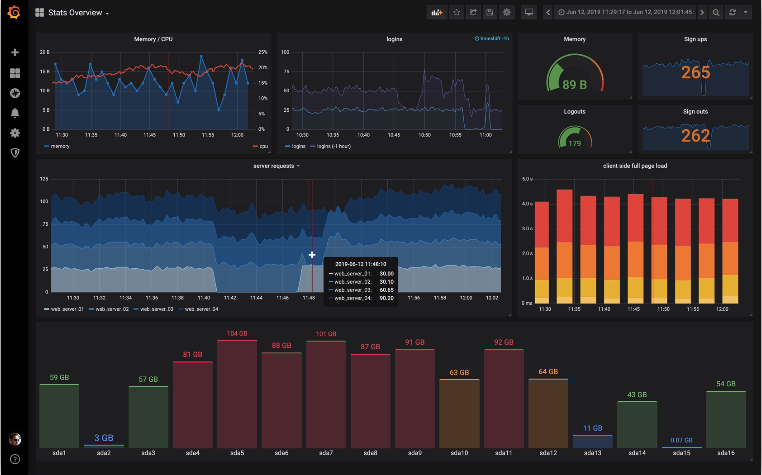
\includegraphics{obrazky-figures/grafana.png}
    }
  \caption{Webové rozhraní aplikace Grafana \cite{grafana}.}\label{pic:grafana}
\end{figure}

%v článku big data processing jsou tři postupy, analytický, matematický, data mining
%Kromě základního přístupu k datům v podobě konzolového rozhraní které nabízí většina databází i

%api rest, ale zmínit přímo napojení na data pomocí SQL-on-Hadoop
%příklad jak to funguje? vkládání a tak?
